\chapter{Identifying impactful fusion genes: fusion expression
  analysis}


\section{Motivation}
Acquisition of increasing numbers of somatic mutations on a rapid
timescale and in a heterogeneous fashion across different cells within
a tumor or pre-tumor tissue, is widespread and occurs in most cancer
types. Resulting mutations are sufficient to induce tumorigenesis and
also to drive tumor progression and metastasis. This is done
classically through the activation of proto-oncogenes and through the
deactivation of tumor suppressor genes.


There are several specific pathways by which mutations can be induced
and several corresponding classes of mutations\cite{stratton_cancer_2009}. One class is
large-scale genomic rearrangement, which involves the breaking and
possible rejoining of multiple-megabase sections of DNA.


When large genomic regions dislocate, they may often rejoin in a
predictable fashion to regions either on other chromosomes or within
the same chromosome (translocations).  If there are genic regions
spanning the genomic breakpoints, RNA messages may be transcribed that
contain two genes from two constituent chromosomes. Such messages, if
translated, become fusion genes (FGs).


Due to fragile regions in DNA, specific FGs may be formed to a
significant extent in certain tissues during
tumorigenesis\cite{yunis_constitutive_1984}. In chronic myeloid
leukemia (CML), a fusion between breakpoint cluster region (BCR) and
Abelson murine leukemia (ABL) virus genes leads to the recurrent
BCR-ABL fusion which is present in a large percentage of CML
patients. This fusion is known to have potential to transform normal
cells into cells with tumor characteristics, and has been successfully
targeted by Imatinib, one of the world’s first successful targeted
therapies in terms of extending patient overall survival time. Several
similar examples have been discovered; identifying FGs is thus of
primary interest \cite{chin_cancer_2011}. 

One goal of major consortium efforts such as The Cancer Genome Atlas
(TCGA)\cite{weinstein_cancer_2013} and The Cancer Cell Line
Encyclopedia (CCLE)\cite{barretina_cancer_2012} is detecting recurrent
fusion genes from different caner types based on sequencing
information. Recently, for example, recurrent receptor tyrosine kinase
fusions were detected in gliomas\cite{_comprehensive_2015}.

One mechanism whereby fusion genes may have impact on tumor tissue is
via the induced expressional deregulation (ED) of the constituents. In particular, a sequence may be placed under the control of regulatory regions that were not originally meant for a sequence, resulting in, for example, the constitutive expression of a growth-factor related protein domain \cite{weinberg_biology_2013}, leading to oncogenesis or tumor progression. 


\section{Existing impact-assessment strategies}
\subsection{Detection}
Typically, fusions are detected from RNA-sequencing (RNA-seq) reads,
which are produced due to its relatively low cost compared to whole
genome sequencing and high interpretability. Several computational
tools to detect fusions from RNA-seq reads exist. Most identify fusion
junctions (FJs), which are the breakpoints of the associated
genomic translocations.


Tools identify FJs in three steps: (1) finding chimeric reads (CRs), which is a single read with two portions aligning to two separate genomic locations, (2) aggregating chimeric reads into candidate fusion junctions through realignment-based grouping, and (3) filtering candidate FJs based on heuristic filters. 

While simple in concept, identifying FJs is a problematically error-prone process. Firstly, incorrect read mapping leads to spurious CRs. Incorrect mapping is often a result of repetitive regions in the genome such as germline segmental duplications. Secondly, even if reads are correctly aligned, false positives may be generated by read-through events, where genomically adjacent genes are erroneously transcribed into one RNA message or reverse transcriptase template-switching events/ trans-splicing. These produce low but detectable baseline levels of fusion genes in wild-type cells, but are usually not of interest in cancer sequencing efforts as they are not causally involved in tumorigenesis, cancer progression, or metastasis\cite{gingeras_implications_2009}. 

Thus, candidate FJs must be filtered aggressively by heuristics based on knowledge of the above. One problem is that it’s not clear exactly which heuristics to use; many heuristics based on ignoring FGs in repetitive regions, for example, may filter real fusions\cite{kumar_identifying_2016}. Another is that given a set of heuristic filters, it’s not clear how to best combine the heuristics in a way that’s generalizable to most FG discovery use cases. This is due in part to the wide range of genomic instability that tumors from different tissues have exhibited. A symptom of this is that Machine learning-based classifiers tuned on representative datasets have issues generalizations to new tumor types. The high false-positive rate stymies further discovery and assessment of FGs. 

FJ identification is also a very computationally-intensive process, as every read must be split in a number of ways and positions and matched against all possible regions of the genome through alignment during CR-finding steps. One of the reasons for this is that existing fusion discovery methods use computationally intensive first-generation alignment algorithms. 

\subsection{Expression quantification}

As ED is a major mechanism by which fusion genes impact tumors and patients, assessing whether an individual fusion detected has also led to ED is a goal for prioritizing fusions for per-patient impact and for further mechanistic study.

Unfortunately, there is no currently established method of doing so in a high-throughput, unbiased fashion. Three methods currently exist:

\subsubsection{Constituent gene summing}

One approach to assessing whether a fusion gene or transcript is expressionally deregulated is by summing the expression estimates of its constituent transcripts. If the sum of these expression estimates substantially deviates from the same quantity in sample(s) without the fusion, it is concluded that the fusion has led to ED.

However, this is inaccurate due to details involving how much of each constituent transcript makes up the fusion. In particular, a fusion gene can consist of the entire transcripts of the constituents bound, or it can consist of as little as a few bases of each gene. This wide discrepancy leads to the lack of robustness of this method without substantial additional human assessment, which is undesirable as the purpose of high-throughput and automated assessment methods is to minimize human input. The presence of large numbers of false-positive fusions exacerbates this necessity of visual inspection as well.

\begin{center}
\begin{figure}\centering
  \parbox{.9\textwidth}{\centering
\noindent 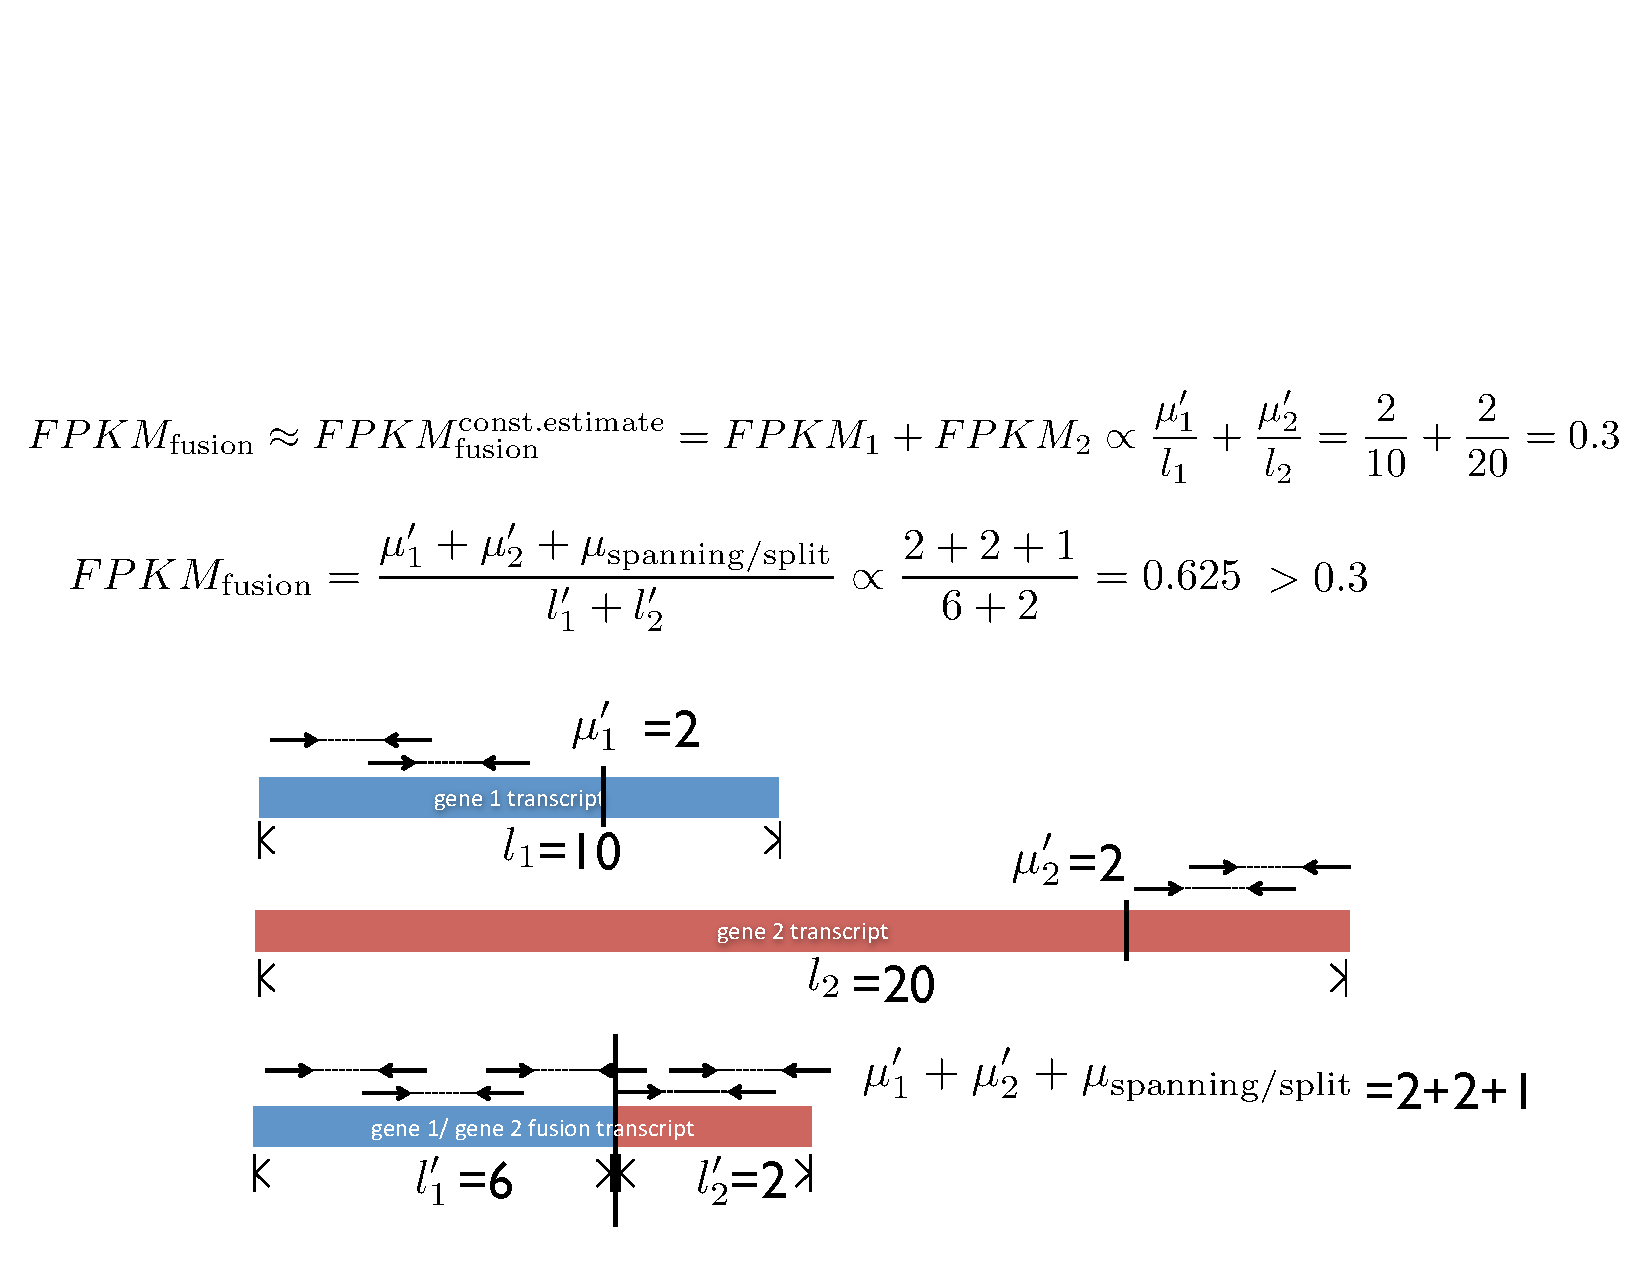
\includegraphics[width=.9\textwidth]{/Users/ijoseph/Documents/Work/Graduate-Thesis/TeX/figures/ch3_1.pdf}
    \caption{Illustration of inaccuracy of constituent summing method ($\mathrm{FPKM}_{\mathrm{fusion}}^{\mathrm{const.estimate}}$) for estimating expression of fusion transcript ($\mathrm{FPKM}_\mathrm{fusion}$), resulting in underestimation by a factor of $2$. $\mu_i \coloneqq$ number of reads aligning to transcript $i$; $l_i \coloneqq$ length of transcript $i$. $\mu_{\text{spanning/split}} \coloneqq$: sum of number of PRs and LRs.}}
\end{figure}
\end{center}


\subsubsection{Per-exon inspection}

A related but distinct method of assessing fusion genes is comparison between fusion-present and fusion-absent samples by visually inspecting the per-exon expression of the constituent transcripts. While not susceptible to the problems of the summing method in terms of misestimation, this is even more labor-intensive as it is completely not automated.

\subsubsection{Counting junction-spanning reads}

One automated approach to assessing fusion expression estimation is by counting the number of reads supporting the fusion junction. In particular, a read can \textit{support} a fusion junction by being a \textit{spanning read} (PR) or \textit{split read} (LR). A PR is a paired-end read wherein one end maps to one transcript and another maps to a genomically distal genomic region, whereas an LR is a read wherein a portions of one read (if applicable) map to at least two distinct genomic regions.

Some method of counting these reads is a common method of prioritizing fusions; however, this is very susceptible to multi-mapping reads. In particular, if a junction region is repeated in another section of the genome, reads could spuriously seem to strongly support a fusion, whereas in reality the reads were produced by different regions altogether. Thus, this method can be inaccurate. One could imagine further difficult-to-set parameters describing heuristics for filtering these reads\cite{mcpherson_defuse:_2011}, but this is a complicated and error-prone process in and of itself.

\subsubsection{Problems with all existing methods of fusion expression quantification}

With all of the above method, a fusions' expression is not directly comparable to the expression of other genes or transcripts. In particular, fusions' expression is not comparable to wild-type constituents' expression, which would be helpful in order to support functional activity of a fusion for prioritization and also for the existence of the fusion. Furthermore, none of the above methods are isoform-specific; all of these merely assess the expression of the fusion gene as a whole, even though isoform-specific expression has found to be impactful in cancer\cite{christofk_m2_2008}\cite{hovanes_-cateninsensitive_2001}\cite{_insulin_2003}.


\section{Method}

Thus, we propose an improved method for isoform-specific FG discovery and quantification from RNA-seq reads.

In short, the method involves three steps, all of which involve k-mer-based pseudoalignment methods: (1) discovering and aggregating LRs and PRs to predict FJs, (2) construction of candidate fusion transcript isoforms (CFTIs) from FJs, and (3) realignment of reads in order to quantify CFTIs along with all transcripts in the transcriptome.

\subsection{Predicting Fusion Junctions}

The first step of the method is to predict fusion junctions based on LRs and PRs. This is achieved using pseudoalignment methods, which in turn involve the splitting of reads into k-mers, the creation of a De Bruijn-graph transcriptome index for alignment, and aggregation of hashed alignment counts per equivalence class, each of which represent a subset of all possible transcripts.

First, reads with ends aligning to discordant equivalent classes are gathered as candidate PRs. Then, these are aggregated along with non-aligning reads (which include LRs) using a De Bruijn-graph alignment format to assemble candidate fusion junction regions. Finally, these regions themselves are pseudoaligned to the transcriptome in order to find candidate fusion junctions.

Note that this step can be replaced by the use of ordinary RNA-seq-read-based fusion finding tools, such as DeFuse\cite{mcpherson_defuse:_2011} or Tophat-Fusion\cite{kim_tophat-fusion:_2011}; results below show data generated by this method.

\subsection{Construction of Candidate Fusion Transcript Isoforms}

Given specific FJs in terms of genomic location, CFTIs are constructed based on enumeration of all possible unique isoforms downstream and upstream of this genomic region. These isoforms can then be added to the alignment index. Note that this can be a De Bruijn-graph-based transcriptomic index\cite{bray_near-optimal_2015} for pseudoalignment, or a Bowtie Burrows-Wheeler-based index \cite{langmead_fast_2012}.

\subsection{Estimating Expression of Fusion Transcripts}
Using the CTFI-appended transcriptome index, the classic generative-model based expression estimation approach is used to estimate the expression of all transcripts, including CFTIs.

Briefly, this model\cite{trapnell_transcript_2010}\cite{roberts_improving_2011}\cite{roberts_fragment_2013} operates via the estimation of parameters representing quantities of interest (transcript interest) and accounts for biases using other parameters, other parameters including per-transcript positional bias and read-composition-based sequence bias.

Importantly, this probabilistic model makes assumptions that assist with the recreation of transcript-wide, isoform specific expression estimation. Crucially, modulo the above biases, the uniform coverage assumption is used in order to deconvolute the extent to which non-junction spanning reads contribute to the expression of the fusion transcript.

The model is a likelihood-based approach which uses hidden data and the expectation-maximization\cite{tipping_mixtures_1999} algorithm to estimate parameters.

The result is an estimation of the expression of all transcripts in the CTFI-appended transcriptome, including, importantly, the CTFIs and their constituents.

\subsection{Checking for Impact of Fusion Transcript}

There are three distinct tests that can be performed for the related states of existence, expressional deregulation, and impact of a FJ and its candidate CTFIs:

\subsubsection{Overall increase in likelihood of model for including fusion transcript}

Since the probabilistic expression model gives a likelihood for a given set of transcripts and a given transcriptome, the likelihood for a fixed transcript set can be seen as a function of a transcriptome. The interpretation of this function is that it will take on a higher value of the transcriptome is more compatible with the sequencing reads; this can be seen as evidence that the transcriptome is the generating transcriptome.


Thus, the likelihood of the model can be compared between a transcriptome with and without CTFIs; this is direct evidence for the existence of a particular FJ and the related CTFIs.

\subsubsection{Decrease in bootstrap variance of constituents when including fusions}

Using the modern Kallisto\cite{bray_near-optimal_2015} expression estimation model, an empirical variance that represents the uncertainty of a particular transcript's expression is estimated. If these quantities decrease for the constituents upon addition of CTFIs, this can be also taken as evidence for FJ and CTFI existence.

\subsubsection{Test of nonzero expression for fusion transcripts}

Given the expression of all transcripts including CTFIs, one can validate the existence of a particular fusion transcript in a sample based on comparing the expression of the CTFI to the expression of its constituents. In particular, if the CTFI has high expression compared to each constituent, this can be seen as evidence for existence of the fusion transcript. However, if no CTFIs of a given FJ are expressed more than any of their constituent transcripts, this can be seen as evidence against the existence of that fusion transcript.

Regardless, this method allows for the identification of expressionally-deregulated fusion transcripts, in the sense that it allows for direct identification of expressional differences. This can be achieved via comparison of the fusion transcript's expression to the expression of constituents in a panel of matched normal cells known to be lacking the relevant FJ in their DNA. One can use formal differneital expression tools to gather significance for such a test, such as Cuffdiff\cite{trapnell_differential_2013} or DESeq\cite{anders_differential_2012}.

\section{Results}

In order to prototype and validate the method, we worked with members of the TCGA LGG AWG. In particular, collaborators at University of California, Santa Cruz and the MD Anderson Cancer Center both ran FJ-discovery software and prioritized samples and fusions for us to assess with our method.

\subsection{Overview of Group Findings}
The full analyses of LGG by the AWG were published in 2015 \cite{_comprehensive_2015}. The major findings, to which the above method contributed, were that there are three molecular categories of LGG that are effective at predicting prognosis. There was great concordance between sequencing datatypes in this regard. Thehe mutation status, obtained through somatic mutations, of the isocitrate dehydrogenase 1 (IDH1) gene plus the presence of chromosome arms 1p and 19q were sufficient to divide patients into three categories: IDH wildtype, IDH mutant with 1p/19q intact, and IDH mutant with 1p/19 deletions.

This was in concordance with clusters obtained via several unsupervised analyses based on DNA methylation, mRNA, copy number and reverse-phase protein assay. Thus, variance between patients ain the genome, epigenome, transcriptome, and proteome showed high concordance.

\subsection{Validation of Method}

Several fusions were detected using DeFuse\cite{mcpherson_defuse:_2011} and PRADA by collaborators in the group. These fusions were detected within IDH mutant samples and were investigated as possibly explaining within-group variation in prognosis based on known attributes of mechanism. One major category of fusions detected were those involving receptor tyrosine kinases, which are which are involved in cell signalling. As part of the mitogenic circuitry, activity of RTKs leads to mitotic cell division. RTKs are often activated via proximity; thus, overexpression is sufficient to induce activation, as it leads to a higher chance of proximity. 

\subsubsection{Case 1: FGFR3-TACC3 Fusion}

First, we studied a patient with a fusion detected between the Fibroblast Growth Factor Receptor 3 and the Transforming, Acidic, Coiled-coil-containing Protein 3 genes (an FGFR3-TACC3 fusion).

This fusion was a good candidate for validation of our method as it has been identified as undergoing fusion-modulated expressional deregulation \cite{parker_tumorigenic_2013}.

\begin{figure}
  \centering 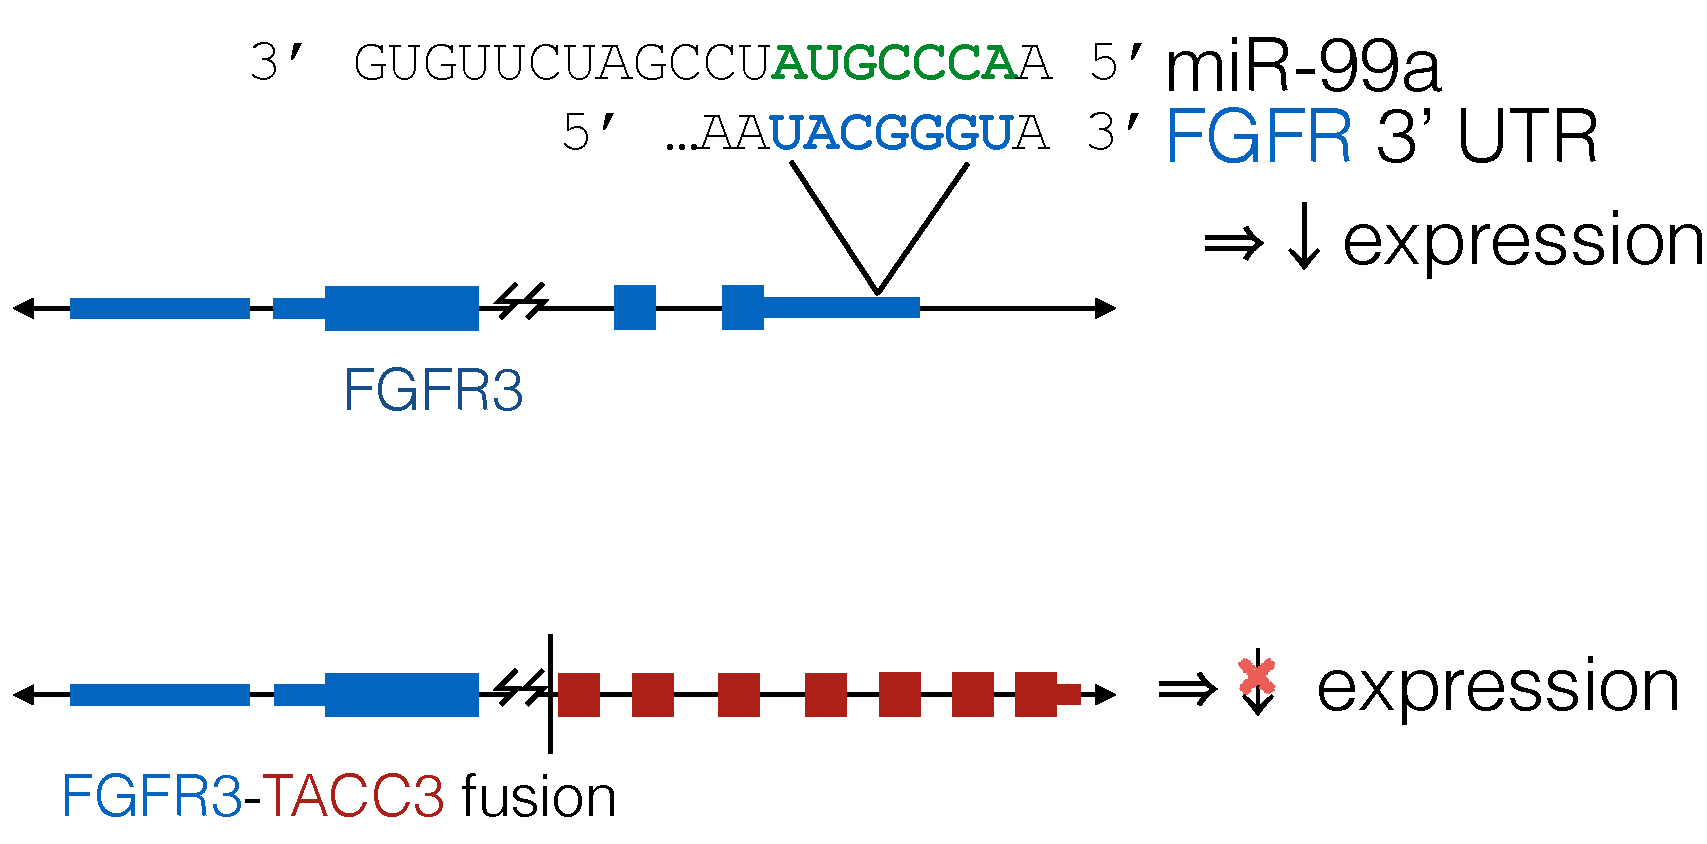
\includegraphics[width=.9\textwidth]{/Users/ijoseph/Documents/Work/Graduate-Thesis/TeX/figures/ch3/miRNA.pdf}
  \caption{Model of deregulation for FGFR3-TACC3
    fusion} \label{threeone}
\end{figure}


The mechanistic model is as follows: the regulation of FGFR3 is based on the annealing of its 3' untranslated region (UTR) to a micro-RNA (miRNA) (miR-99a, in particular) (see figure \ref{threeone}). When miR-99a anneals to the FGFR3 transcript, the transcript is marked for degradation. Thus, FGFR3's expression is downregulated based on its 3' UTR region. However, the fusion is formed such that the FGFR3 constituent lacks its 3' UTR, and therefore loses its wild-type regulatory mechanism. This leads to the temporally and spatially ectopically elevated expression of the FGFR3 sequence, leading to mitosis via mechanisms explained above.


Upon applying the method using eXpress as our expresion quantification module\cite{roberts_streaming_2013} on this specific paper, we were able to validate the results.

\begin{figure}
  \centering 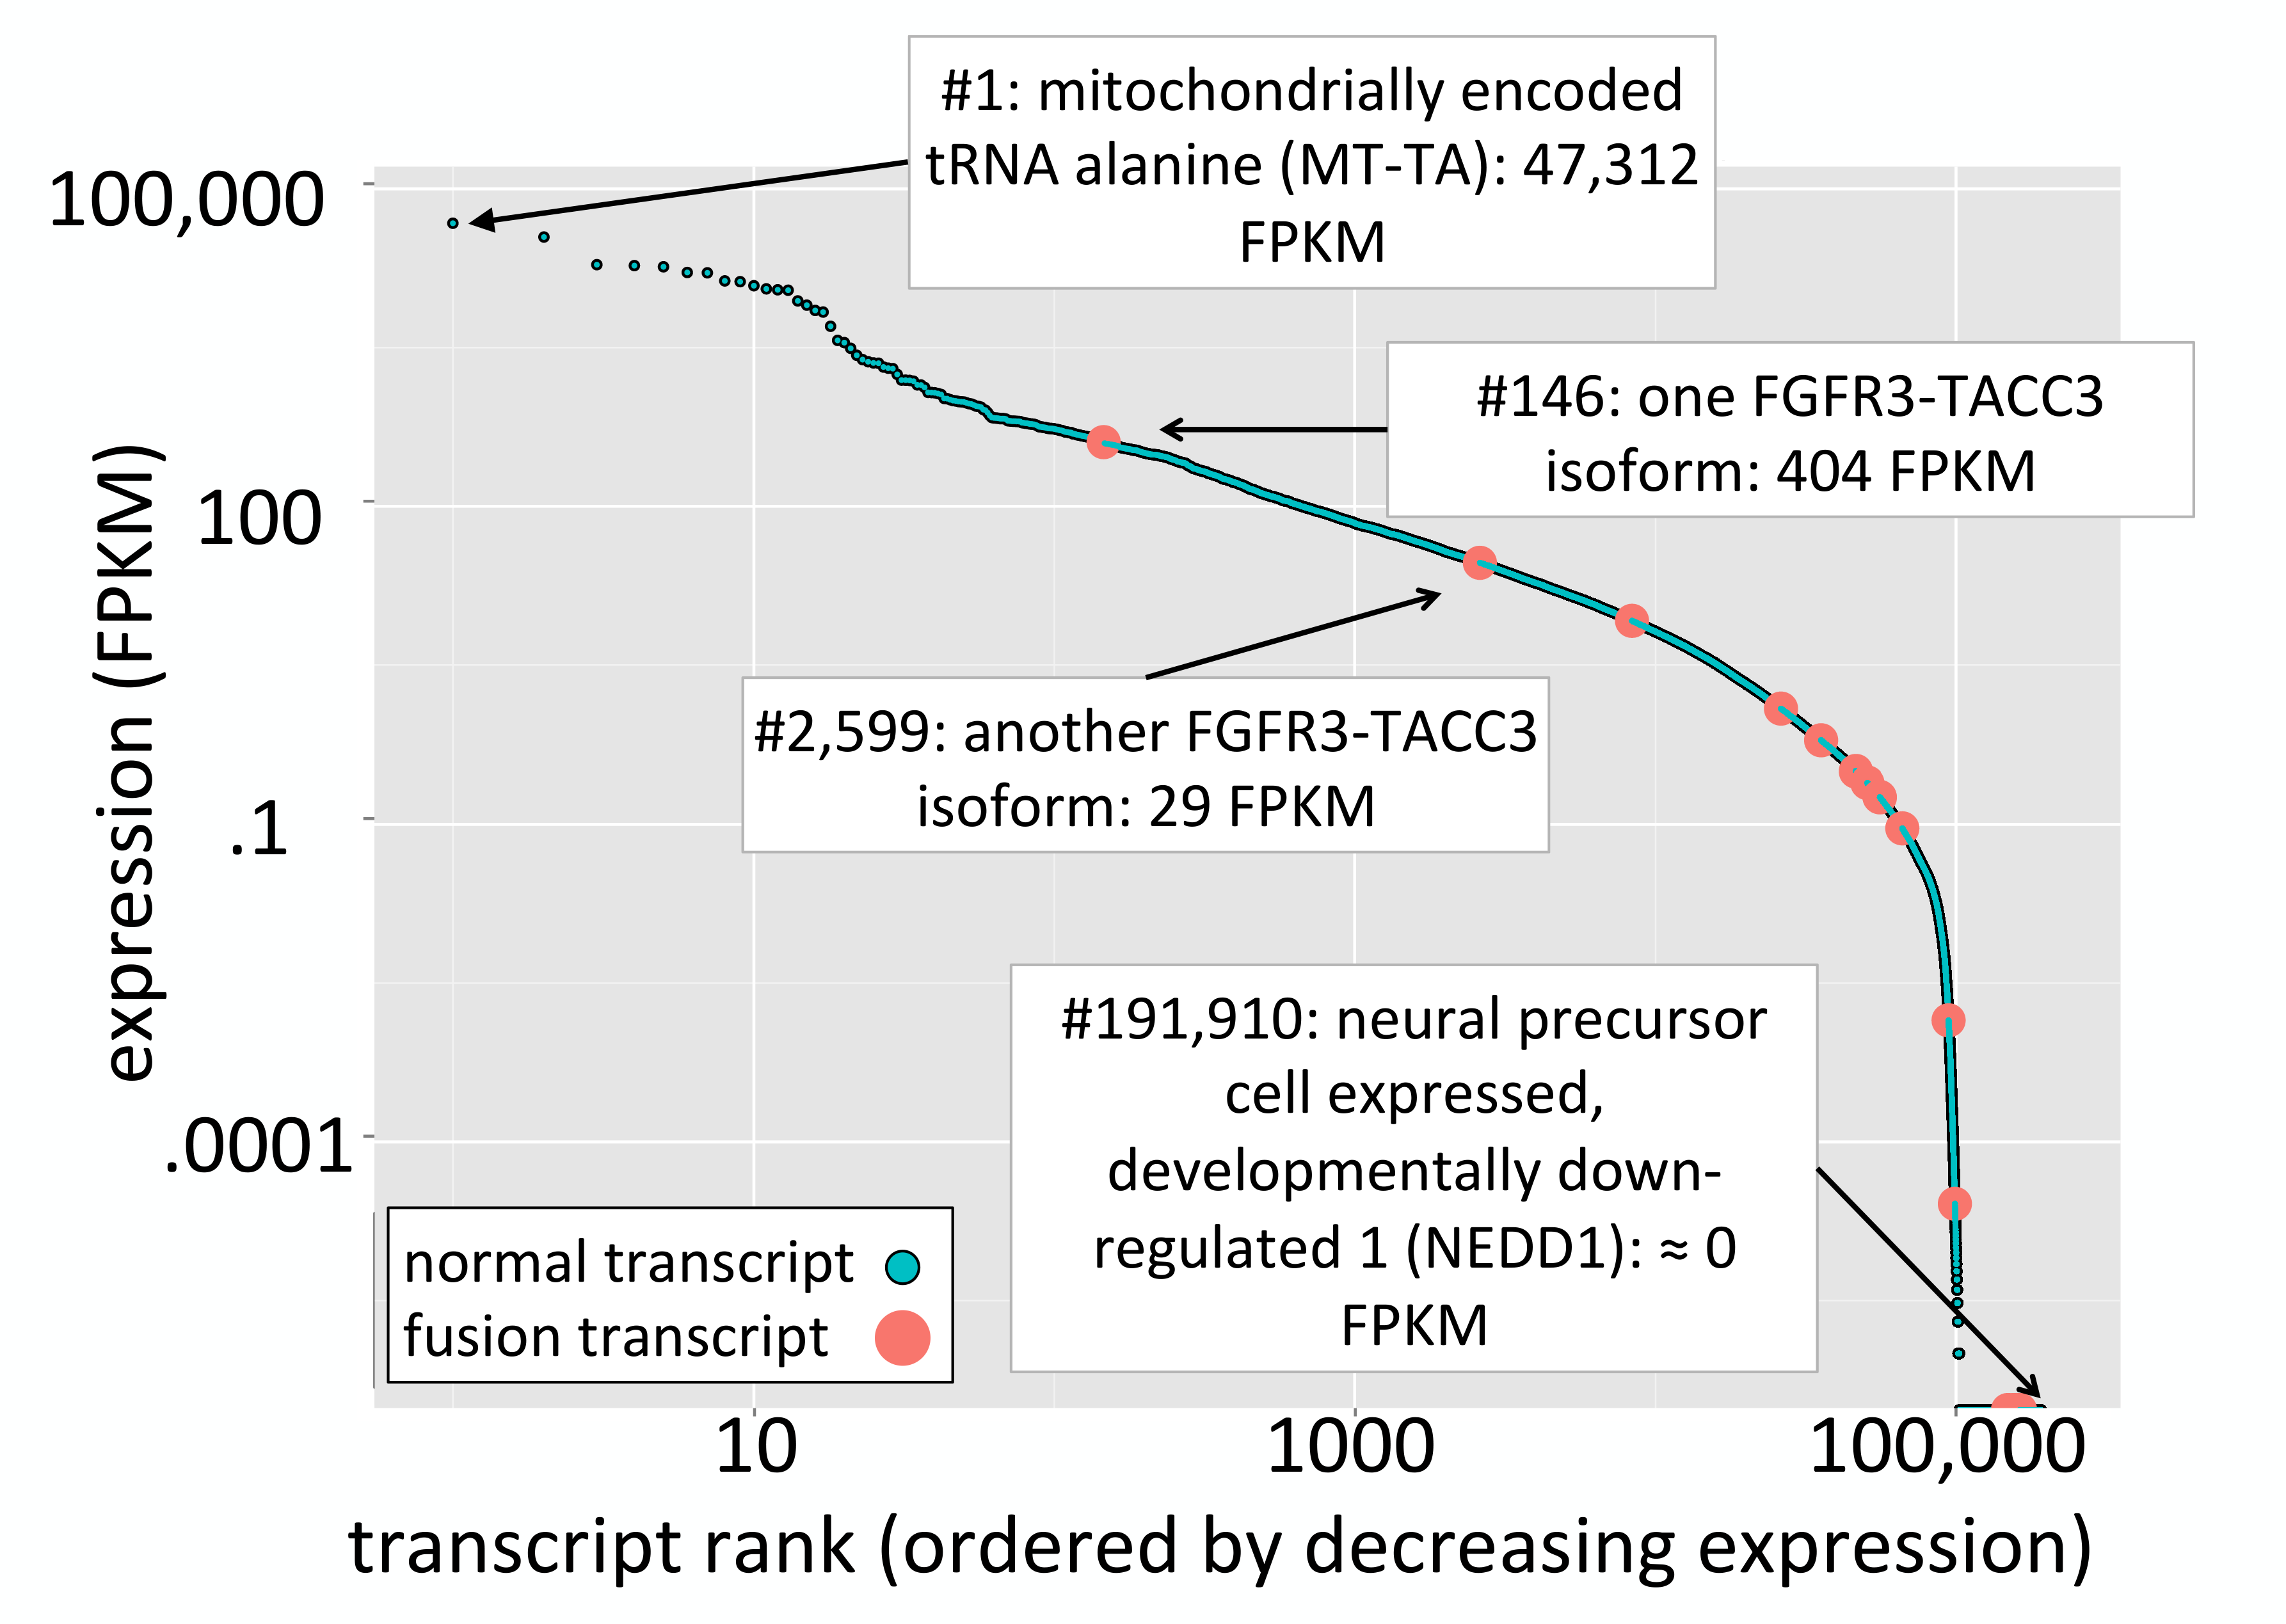
\includegraphics[width=.9\textwidth]{/Users/ijoseph/Documents/Work/Graduate-Thesis/TeX/figures/ch3/all_transcripts.png}
  \caption{Expression of all transcripts in transcriptome for
    individual} \label{threetwo}
\end{figure}


Firstly, we noted that isoforms of FGFR3-TACC3 fusion transcripts were among the highest-expressed transcripts in the transcriptome (see figure \ref{threetwo}). This was a sanity check offering consistent evidence with the ectopically high expression of FGFR3-TACC3.


\begin{figure}
  \centering 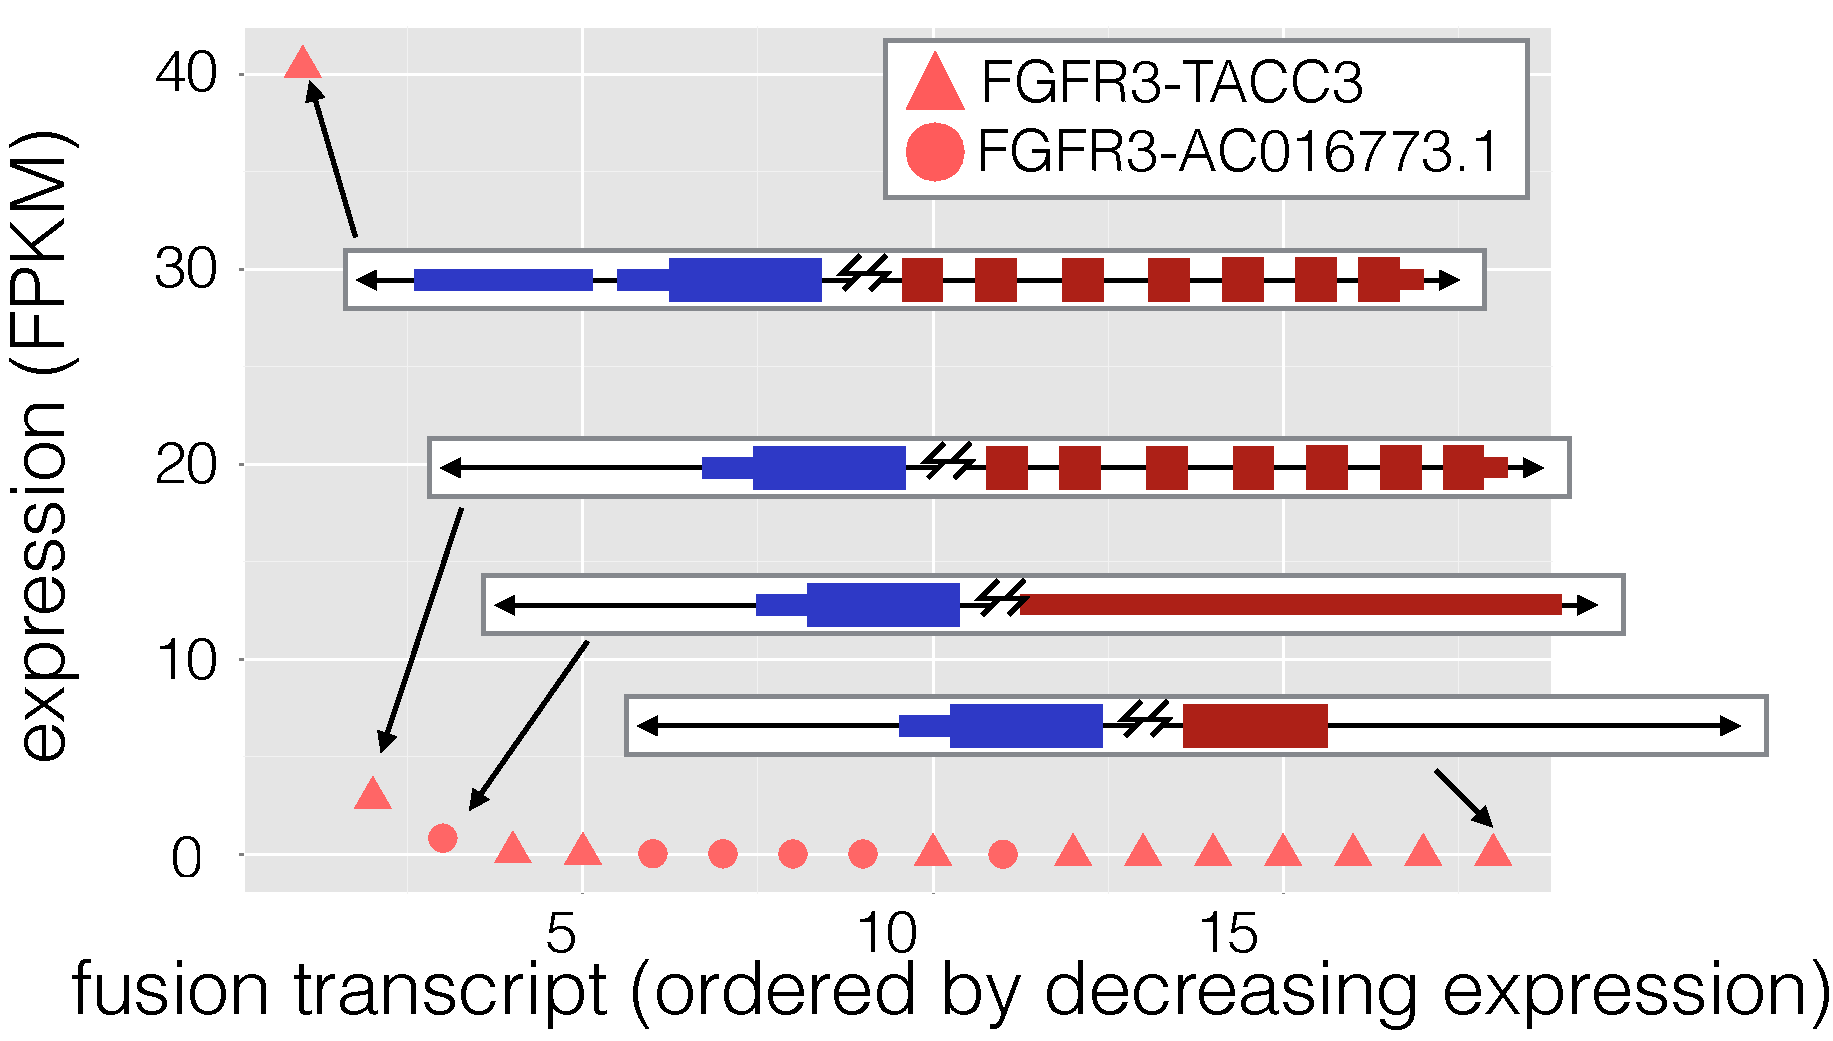
\includegraphics[width=.9\textwidth]{/Users/ijoseph/Documents/Work/Graduate-Thesis/TeX/figures/ch3/just_fusions.pdf}
  \caption{Expression of fusion transcripts in the transcriptome showing isoform-resolution expression discrimination} \label{threethree}
\end{figure}



Secondly, we noted that we were able to differentiate between the expression of fusion transcript isoforms. In particular, we found that one isoform's expression dominated the expression of all others (see figure \ref{threethree})


Thirdly, we noted the correct assessment of the FGFR3-TACC3 fusion transcript isoform versus an FGFR3-AC016733.1 transcript, also formed based on the same FJ (see figure \ref{threethree}).


\begin{figure}
  \centering 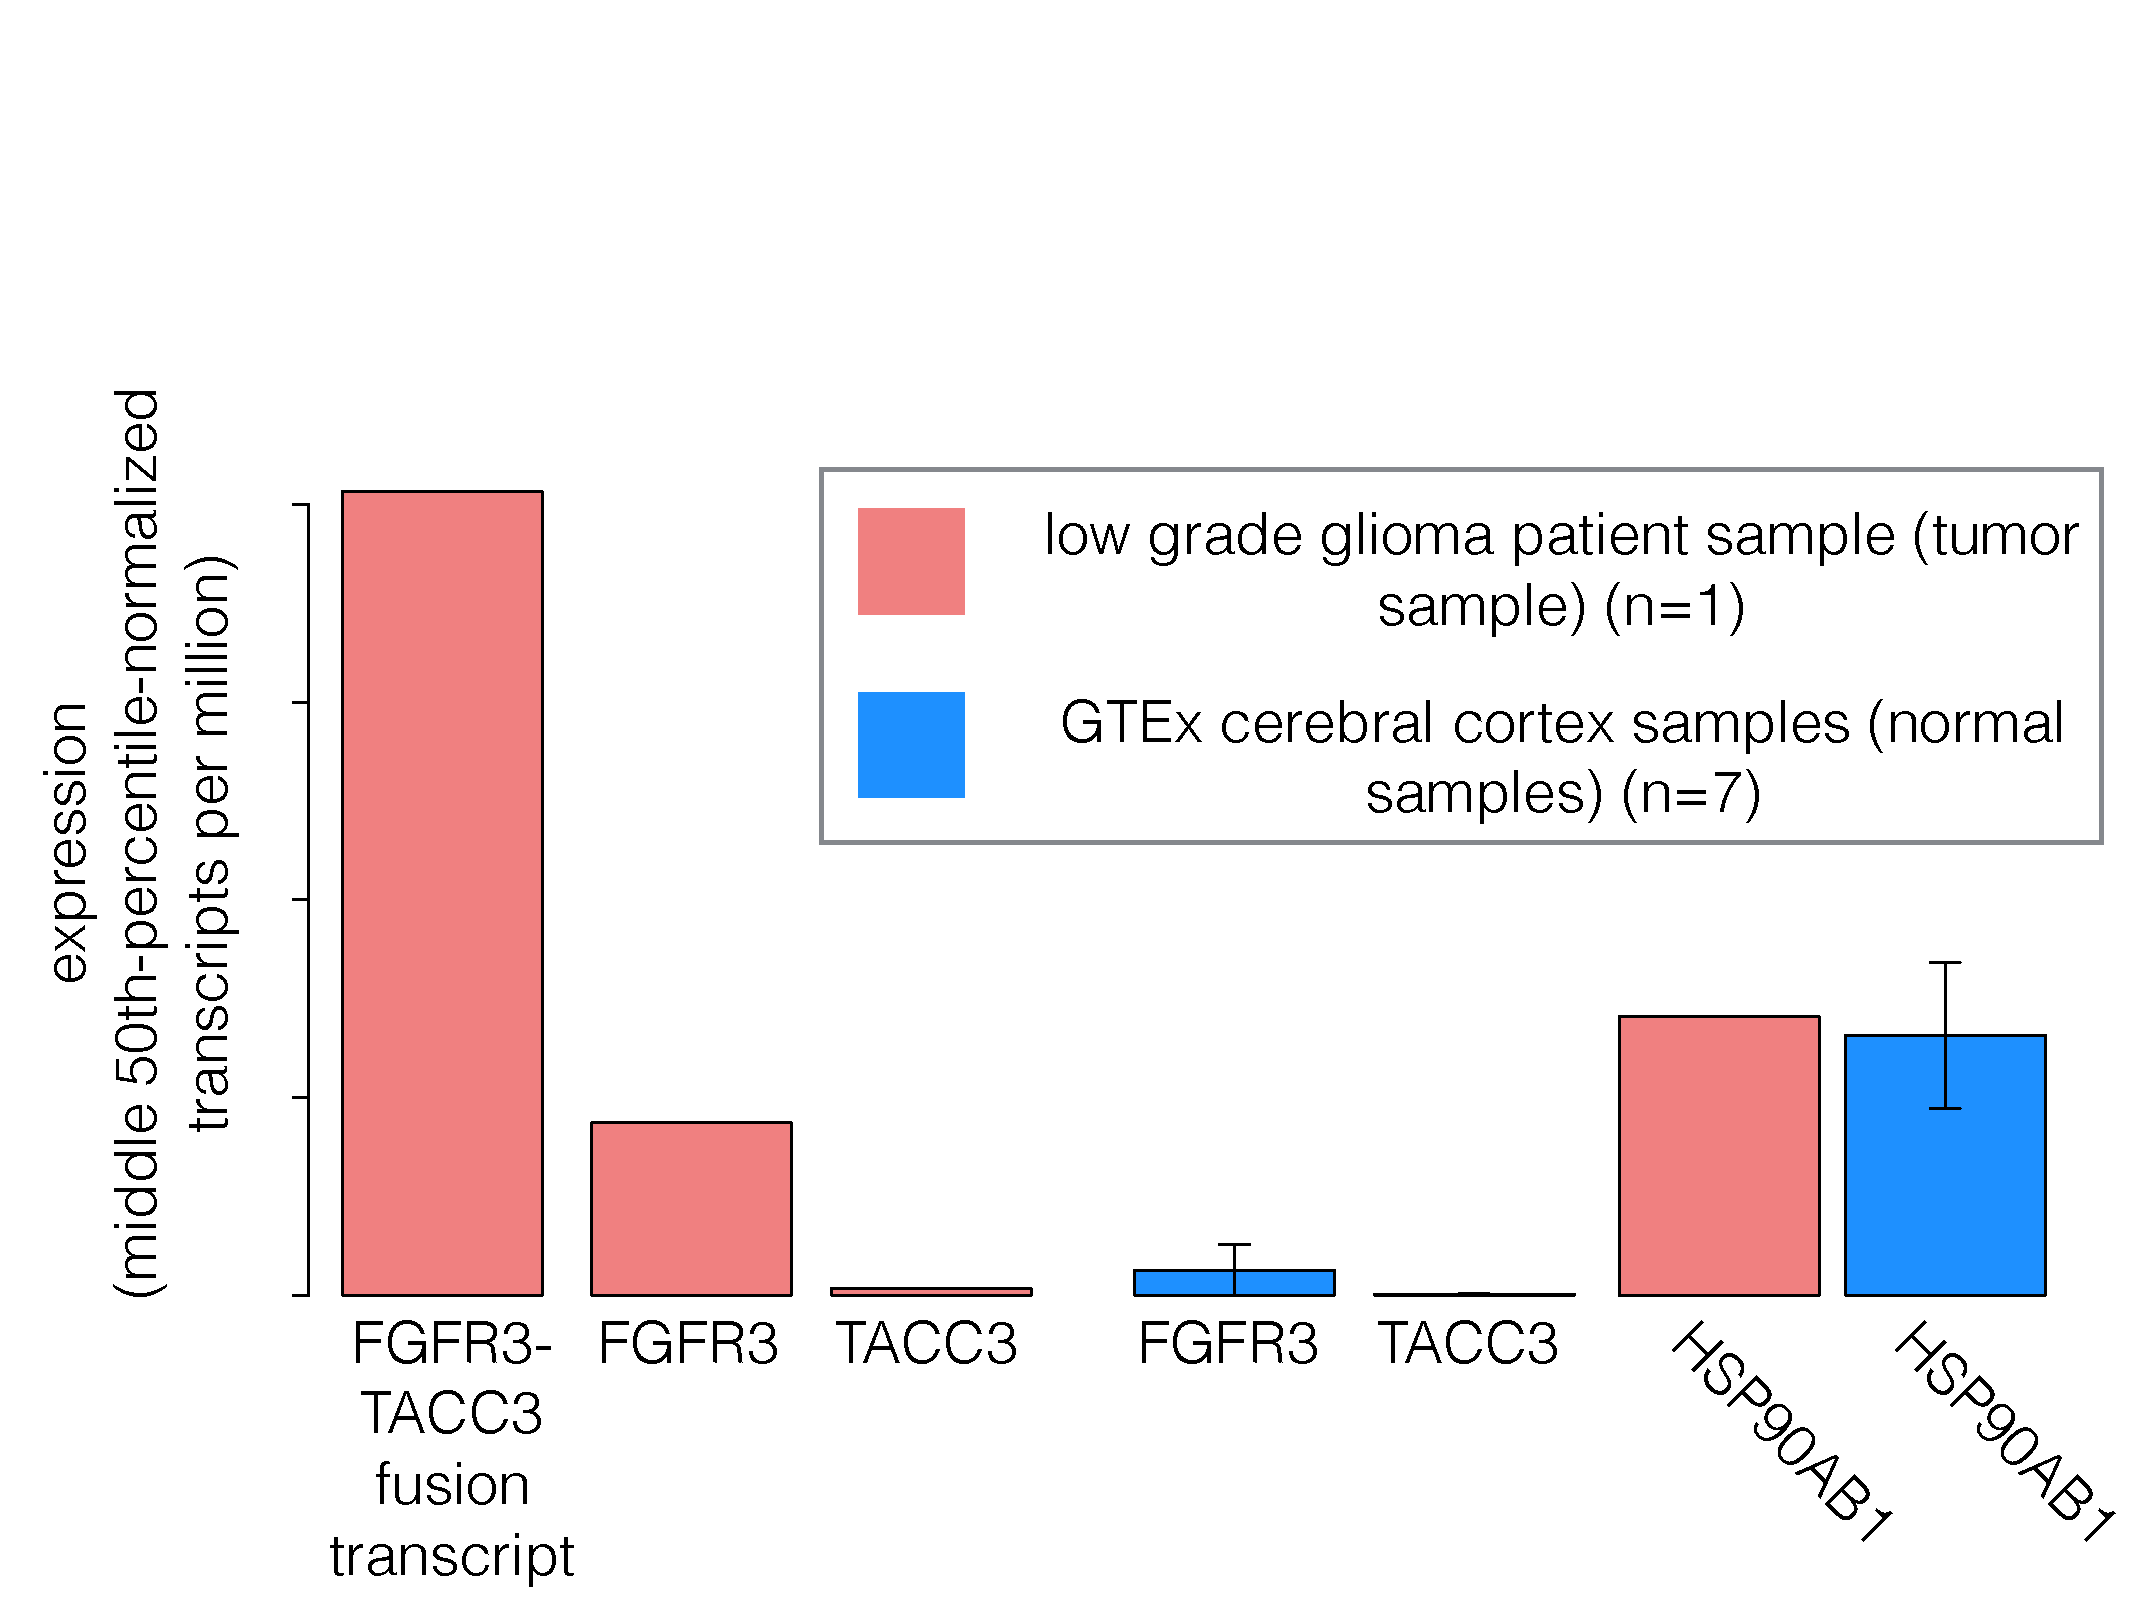
\includegraphics[width=.9\textwidth]{/Users/ijoseph/Documents/Work/Graduate-Thesis/TeX/figures/ch3/comparison.pdf}
  \caption{Expression of fusion transcript is higher than constituents in same cell and in related normal cells}\label{threefour}
\end{figure}


Finally, we validated that the expression of the fusion transcript was higher in expression than its constituents in the same cell (figure \ref{threefour}) , finding that the fusion transcript's expression was more than 3 times the expression of FGFR3 and 100 times the expresion of the TACC3 transcript (see figure \ref{threefour}).

We also compared the fusion transcripts' expression to its constituents in matched normal tissue. This allowed for further evidence of the fusions' leading to expressional deregulation.

In order to make the comparison between the sample of interest and cerebral cortex samples from the Genotype-Tissue Expression project (GTEx)\cite{lonsdale_genotype-tissue_2013}, we transformed expression estimates from fragments per kilobase per million-reads-mapped (FPKM) to transcripts per million (TPM), then applied middle-50th-percentile-normalization\cite{_what_2014}. We validated this normalization by using a housekeeping gene, heat-shock protein, 90-kilodaltons, alpha, class b, member 1 (HSP90AB1), for which strong evidence exists of relatively stable expresion temporally, spatially, and inter-cell-type. We saw that the expression in the sample of interest of HSP90AB1 was similar to that of the normal tissue.

We validated that the expresson of the highest-expression FGFR3-TACC3 fusion transcript isoform was much higher than that of its constituents the matched normals -- on the order of 10 to 1000 times higher.

\subsubsection{EGFR-SEPT14 Fusion}

We also studied a fusion between the epidermal growth factor receptor (EFGR) and septin 14 (SEPT14) genes (EGFR-SEPT14 fusion). EGFR is another RTK with similar activity to FGFR3, and was thus another candidate for a fusion having similar oncogenic properties to the FGFR3-TACC3 fusion, although unknown in its ability to expressionally deregulate. EGFR3-SEPT14 is also known to have oncogenic properties in glioblastoma, which is equivalent to grade IV glioma and related as a progression result to LGGs\cite{_omim_2016-1}. 

Once again, we noticed that the expression of the fusion transcripts were above their constituents in many cases (see figure \ref{threefive}). This suggests expressional
deregulation occurred for this fusion.


\begin{figure}
  \centering 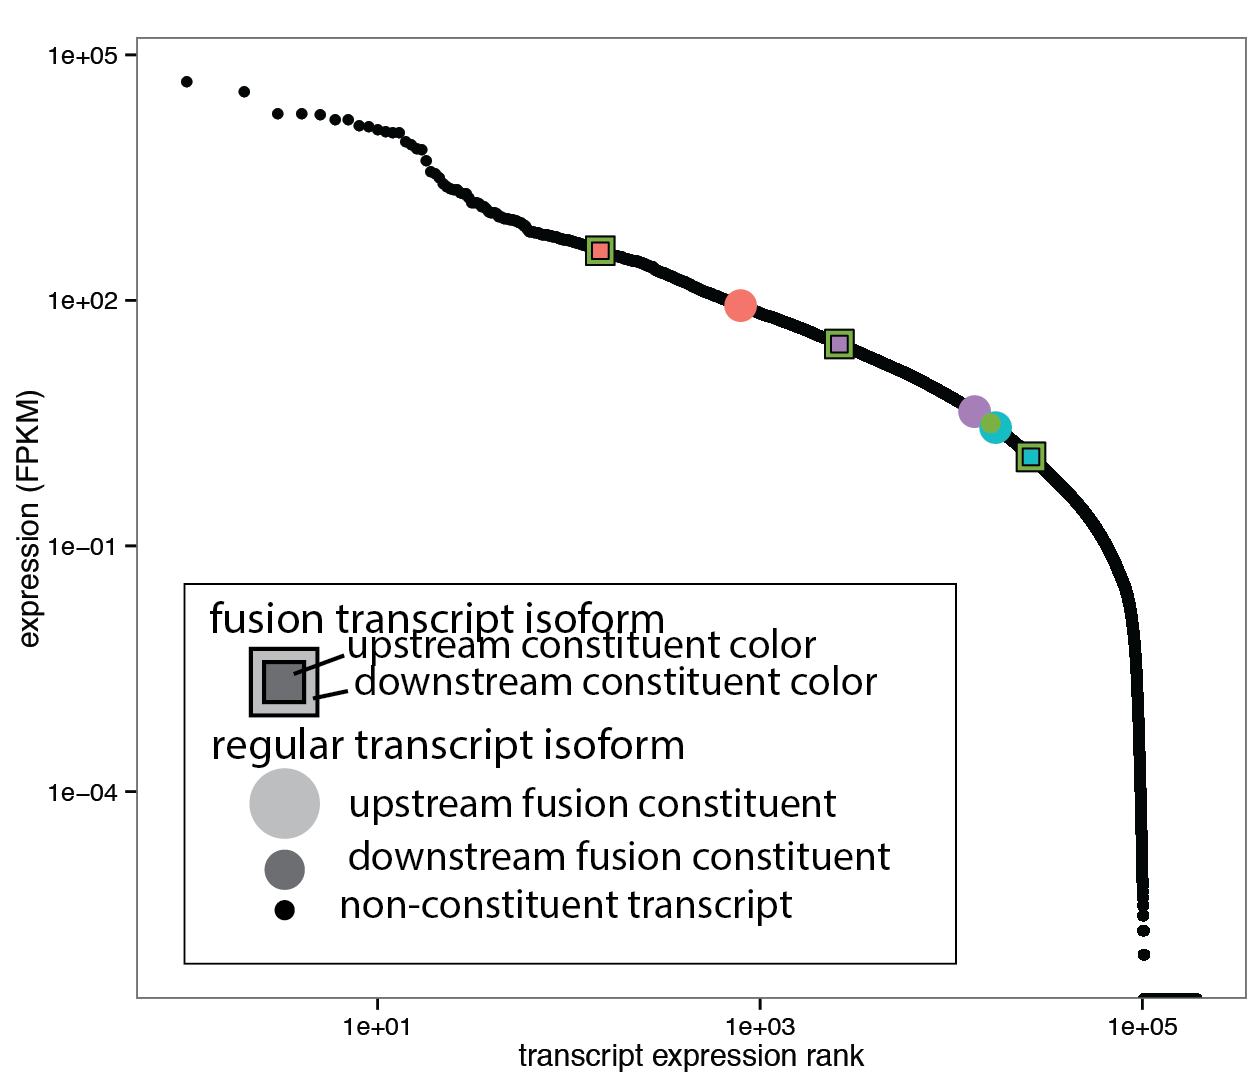
\includegraphics[width=.9\textwidth]{/Users/ijoseph/Documents/Work/Graduate-Thesis/TeX/figures/ch3/3_last_2.png}
  \caption{Expression of all transcripts in patient with EGFR3-SEPT14
    fusion} \label{threefive}
\end{figure}

\section{Discussion}

\subsection{Outlook}
The validation of a known expressionally-deregulated fusion and the identification of a candidate expressionally-deregulated fusion is promising that the method will be useful at identifying expressionally-deregulated fusions in the future based on the metric of assessing the expression of the fusions to be significantly higher than their constituents.

\subsection{Future Work}
  
Much future work could be done on this method; firstly, one could create a formal statistical test of the expression of a fusion transcript being higher than its constituents (a) within sample and (b)a matched panel of normals. This would expedite the identification of expressionally deregulated fusions and would complete the requirement for not requiring manual user assessment of results.

Secondly, one could expand on this method to both identify FJs and lead to their expression. Currently, this is being done by Shannon Hateley and Dr. P\'{a}ll Melsted, Ph.D. by adapting the Kallisto pseudoalignment algorithm\cite{bray_near-optimal_2016} to identify FJs based on discordantly-mapped k-mers.

Thirdly, one could also use modern k-mer-mapping-based expression methods to achieve the expression quantification portion, which are much faster and would be useful as well for providing variance-based evidence for fusion existence.

Fourthly, one could integrate this into one tool, such that pipelining, which is a tedious and error-prone process, would not have to be implemented by the user.









